\documentclass[11pt]{article}
\usepackage[T1]{fontenc}
\usepackage[margin=0.85in]{geometry}
\usepackage{amsmath,amssymb,amsthm,booktabs,tikz}
\usepackage[hidelinks]{hyperref}
\newtheorem{theorem}{Theorem}
\newtheorem{corollary}[theorem]{Corollary}
\newcommand{\Q}{\mathbb Q}
\newcommand{\F}{\mathbb F}
\newcommand{\ord}{\operatorname{ord}}
\title{Small auxiliary primes for the Adleman--Lenstra construction after Wesolowski}
\author{AI-produced mathematical study (GPT-6.2 Astra)}
\date{22 November 2026}
\begin{document}
\maketitle
\begin{abstract}
Adleman and Lenstra construct a degree-$r$ finite field over $\F_p$ from a prime $\ell\equiv1\bmod r$ at which $p$ is a non-$r$th power.
For fixed odd prime $r$, Dirichlet GRH alone supplies a single table of primes of size $O_r(\log X\log\log X)$ which works for every $X<p\le2X$ with $O_r(\sqrt X\log\log X)$ exceptions.
A larger table with entries at most $(\log X)^{1+\epsilon}$ leaves $O_\epsilon(\sqrt X)$ exceptions.
For an individual higher-valuation input, a specialization of Wesolowski's ray-class theorem gives an explicit $O(r^2\log^2(rp))$ bound under one additional Hecke zero-location hypothesis.
The finite-table estimates were checked independently by a second GPT-6.2 Astra instance. No human review is recorded.
\end{abstract}

\section{Two directions of variation}
Let $r,p$ be distinct primes with $r$ odd. Call a prime $\ell\ne p,r$ a witness if
\[
 \ell\equiv1\pmod r,\qquad p^{(\ell-1)/r}\not\equiv1\pmod\ell.
\]
The residue of $p$ generates the order-$r$ quotient of $(\mathbb Z/\ell)^\times$.
Hence $p$ is inert in the degree-$r$ subfield of $\Q(\zeta_\ell)$.
The Gaussian-period algorithm of Adleman--Lenstra constructs a degree-$r$
irreducible polynomial over $\F_p$ in time polynomial in $\ell$ and $\log p$
\cite[Algorithm A and Lemma 6]{AL}.
The hypothesis $A_D$ below is RH for the primitive Dirichlet $L$-functions, including RH for $\zeta_{\Q}$.
Tang already gives a deterministic polynomial-time construction from every
promised prime-power order \cite[Theorem 1.1]{Tang}. Tang's Lemma 2.1 obtains
the stronger witness condition $\ell\equiv1\bmod12r$ in its stated range
$p>\max(n,3)$, $r\le n$, using a uniform zero-free strip for Dedekind zeta
functions. Here the question is what the Dirichlet result alone contributes to
the original search.

\begin{figure}[h]
\centering
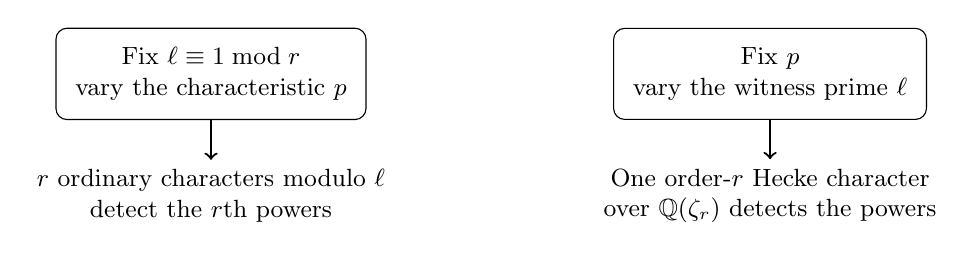
\begin{tikzpicture}[x=1cm,y=1cm, every node/.style={align=center,font=\small}]
\node[draw,rounded corners,inner sep=7pt] (a) at (0,1) {Fix $\ell\equiv1\bmod r$\\vary the characteristic $p$};
\node[draw,rounded corners,inner sep=7pt] (b) at (7.1,1) {Fix $p$\\vary the witness prime $\ell$};
\node (c) at (0,-0.55) {$r$ ordinary characters modulo $\ell$\\detect the $r$th powers};
\node (d) at (7.1,-0.55) {One order-$r$ Hecke character\\over $\Q(\zeta_r)$ detects the powers};
\draw[->,thick] (a)--(c);
\draw[->,thick] (b)--(d);
\end{tikzpicture}
\caption{The same modular test has a different coefficient field for its characters when the variable prime changes. Theorems 1 and 3 quantify the two searches.}
\end{figure}

\begin{theorem}\label{average}
Assume $A_D$. For fixed odd prime $r$ and sufficiently large $X$, a single table of
$k=\lceil\log X/(2\log r)\rceil$ primes $\ell\equiv1\bmod r$, each
$O_r(\log X\log\log X)$, supplies a witness for every prime $X<p\le 2X$
with $O_r(\sqrt X\log\log X)$ exceptions. Both claims hold with
$\ell\equiv1\bmod 12r$. The table can be constructed by deterministic enumeration.
\end{theorem}

\begin{proof}
We give the conductor dependence. Fix a nonnegative smooth compactly supported
weight $W$ on $(0,\infty)$ with $W\ge1$ on $[1,2]$. For a primitive Dirichlet character $\psi$ of conductor $f$, the smooth explicit formula under $A_D$ gives
\[
 \sum_{n\ge1}\Lambda(n)\psi(n)W(n/X)
 ={\bf1}_{\psi=1}X\widehat W(1)+O_W(\sqrt X\log(2f)).
\]
Indeed each nontrivial zero contributes $X^\rho\widehat W(\rho)$.
Integration by parts gives cubic decay in height. The zero count on the unit band at $t$ is $O(\log(2f(2+|t|)))$. The integral on $\Re s=-1/2$ and trivial-zero terms are $O_W(\log(2f))$, by the functional equation; see the comparable smooth formula in \cite[Lemma 11.2]{PF}.
For a character modulo $Q$ induced by $\psi$, the deleted prime powers cost
$O_W(\log(2Q))$: at each $\ell\mid Q$ there are $O_W(1)$ relevant powers in the rescaled support. Here $\widehat W$ denotes the Mellin transform.

Put $Q=\prod\ell$. The subgroup of $r$th powers in $(\mathbb Z/\ell)^\times$
has indicator $r^{-1}\sum_{\chi^r=1}\chi$ away from $\ell$. Multiplication and CRT give the joint
indicator as the average of $r^k$ distinct characters modulo $Q$; precisely one
is principal. Its weighted sum is nonnegative also on prime powers, and is zero
at primes dividing $Q$. Dividing by $\log X$ bounds the exceptional prime count by
\begin{equation}\label{raw}
 O_W\left(\frac{X}{r^k\log X}
       +\frac{\sqrt X\log(2Q)}{\log X}+k\right).
\end{equation}
The last term permits tests that coincide with the input prime. No character
expansion is performed by the field algorithm. Choosing the first $k$ primes in
the fixed progression gives maximum entry $O_r(k\log(2k))$ by the prime number
theorem for progressions. Then $\log Q=O_r(k\log(2k))$ and $r^k\ge\sqrt X$.
\end{proof}

\begin{corollary}\label{square}
For fixed $r$ and $\epsilon>0$, the table of all primes $\ell\equiv1\bmod 12r$
up to $Y=(\log X)^{1+\epsilon}$ leaves $O_{\epsilon}(\sqrt X)$ exceptional
primes $X<p\le2X$ under $A_D$, for $X$ sufficiently large in $r,\epsilon$.
\end{corollary}
\begin{proof}
Write $k$ for the number of tests and take
$m=\lceil\log X/(\epsilon\log\log X)\rceil$. Choose one order-$r$ character
at each prime. Form $\mathcal C$ from the products of the chosen characters
over each $m$-element subset, considered on integers coprime to $Q$.
Distinct subsets have distinct primitive conductors, hence distinct characters.
For fixed $r$, $k\asymp_r Y/\log Y$, so
$\log(k/m)=\epsilon\log\log X+O_{r,\epsilon}(1)$ and
$M=|\mathcal C|=\binom{k}{m}\ge(k/m)^m\ge\sqrt X$ eventually.

On the exceptional primes the squared modulus of
$M^{-1}\sum_{\chi\in\mathcal C}\chi(p)$ is one.
Use the primitive product on each subset, including at integers divisible by unused test primes.
Each term $\chi\bar\chi'$ of the expanded square has modulus at most $Y^{2m}$.
Diagonal pairs alone are principal. The same smooth formula yields
$O_W(X/(M\log X)+\sqrt X[1+2m\log Y]/\log X)$.
Here $Y<X$ eventually. The square is nonnegative on all integers, which justifies passing from its weighted sum to the prime count.
\end{proof}

\paragraph{Many extension degrees at once.}
The prime search underlying Theorem~\ref{average} is uniform.
For a modulus $b=r$ or $12r$, character orthogonality applied to a nonnegative smooth weight supported in $(1,2)$ gives a weighted prime count in the class $1\bmod b$ of
$cY/\varphi(b)+O(\sqrt Y\log(2b))$.
The terms at powers of exponent at least two are $O(\sqrt Y)$ by the elementary Chebyshev bound. Thus the first $k$ entries are at most an absolute constant times
\[
  (r\log(2r))^2+rk\log(2rk).
\]
Choose a sufficiently large constant to dominate the error and to make the prime count at least $k$. For each fixed $B>0$, summing \eqref{raw}
over prime $r\le(\log X)^B$ excludes $O_B(\sqrt X(\log X)^B\log\log X)$ input
primes. The character-average proof applies also to $r=2$.
For all remaining $p$ this supplies all the congruence tests up to
that degree, with entries polynomial in $\log X$.
In the table branch of OpenAI's algebraic prime-field algorithm, Theorem~1.2 and Proposition~10.1 \cite{PF}, these are its required inputs.
This conclusion concerns almost all characteristics; a uniform algorithm for
arbitrary $p$ using only the Dirichlet zero hypothesis remains a separate question about the proof.

\section{A fixed characteristic and its character conductor}
Let $s=\ord_r(p)$ and suppose $r^2\mid p^s-1$. Put
$K=\Q(\zeta_r)$, $F=\Q(p^{1/r})$, and $E=KF$.
Eisenstein at a prime over $p$ gives $[E:K]=r$.
The permutation action on the roots is the affine group
$G=\F_r\rtimes\F_r^\times$. Its degree-$r$ permutation representation is
$1\oplus\operatorname{Ind}_{\F_r}^{G}\theta$ for any nontrivial character
$\theta$ of the translation subgroup. This follows from its transitive
action on the nontrivial characters of $\F_r$, or by comparing character values.
Viewed by class field theory as a Hecke character of $K$, it satisfies
\[
 L_K(s',\theta)=\zeta_F(s')/\zeta_{\Q}(s'),\qquad
 \zeta_E(s')=\zeta_K(s')L_K(s',\theta)^{r-1}.
\]
These are all-prime identities. The first factor is entire by Hecke's theorem for
nontrivial characters. Thus under $A_D$, RH for $\zeta_F$ supplies RH for
$L_K(s',\theta)$, while the abelian extension $K/\Q$ supplies RH for $\zeta_K$.

\begin{theorem}\label{weso}
In the higher-valuation case above, assume $A_D$ and RH for $\zeta_F$. There is a witness
\[
 \ell\le
 \left(2.71\big((r-2)\log r+(r-1)\log p\big)
     +1.38\,\frac{r-1}{s}+4.13\right)^2.
\]
\end{theorem}
\begin{proof}
Since $s\mid r-1$ and $r\nmid(r-1)/s$, the valuation criterion is equivalent to
$p^{r-1}\equiv1\bmod r^2$. In $\Q_r^\times$ split the unit $p$ into its
Teichm\"uller part and its factor in $1+r\mathbb Z_r$. The $r$th power map
is invertible on the first factor. On the second, the $r$-adic logarithm
identifies its image with $r^2\mathbb Z_r$. It follows that $p$ is an $r$th
power in $\Q_r$. The unique prime of $K$ above $r$ therefore splits completely
in $E/K$. Each prime over $p$ is totally and tamely ramified by Eisenstein.
Other finite primes are unramified by the polynomial discriminant. Hence the
conductor of $\theta$ is $p\mathcal O_K$, with $(r-1)/s$ distinct factors.
In particular $|D_K|N(p\mathcal O_K)=r^{r-2}p^{r-1}$.
This agrees with the classical absolute discriminant of $F$
\cite[Lemma 3.1(ii)]{Holmes}.

Apply Wesolowski's Theorem~1.1 \cite{W} to this modulus and the whole ray class
group. His proof in \S3 uses the primitive $L$-functions of the characters
of the quotient by the chosen subgroup and their products with $\theta$;
for the full subgroup these functions are exactly $\zeta_K$ and $L_K(\cdot,\theta)$.
The field is totally imaginary, so the infinite modulus is empty.
The theorem gives an unramified degree-one prime ideal with $\theta\ne1$ within
the stated bound. Its rational prime is different from $p$ by the modulus,
and from $r$ by complete splitting at $r$. Degree one in $K$ means
$\ell\equiv1\bmod r$. Nontrivial Frobenius in $E/K$ is precisely the displayed
power test.
\end{proof}

\paragraph{A fixed-width zero-free strip.}
There is also a uniform polynomial witness bound for all odd $r\ne p$ if
$A_D$ holds and every nontrivial zero of $\zeta_F$ has real part at most
$1-\delta$, for a fixed $0<\delta\le1/2$. Put $H=r\log(2rp)$ and use a
nonnegative smooth weight supported in $(1,2)$ with integral $c>0$. Write
$\Psi_L(x)$ for the weighted von Mangoldt sum over ideals of $L$.
Logarithmic differentiation of the zeta identity above gives
\[
 \Psi_K(x)-r^{-1}\Psi_E(x)
 =(1-r^{-1})\{\Psi_K(x)-\Psi_F(x)+\Psi_\Q(x)\}
 =(1-r^{-1})cx+O(Hx^{1-\delta}).
\]
The smoothed formula follows as in \cite[Lemma 11.2]{PF}, since
$\log|D_F|\le r\log r+(r-1)\log p$ by the polynomial discriminant.
In the absence of a witness in $(x,2x)$ each unramified degree-one prime
of $K$ there splits completely in $E$, cancelling in the left side.
Discarding the remaining nonpositive $E$ terms bounds that side by
$O(r\sqrt x\log(2x))$ from higher residue degrees, prime powers, and the
ramified primes $r,p$, as in \cite[Lemma 2.1]{Tang}.
Choosing $x=C_\delta H^{1/\delta}$ makes both errors less than a quarter
of the main term for a sufficient fixed $C_\delta$. This proves
$\ell\ll_\delta (r\log(2rp))^{1/\delta}$ for the original $1\bmod r$ search.
Cureton--Thorner's stated uniform $31/32$ bound supplies $\delta=1/32$.
This application consumes the strip rather than deducing it from $A_D$.

\paragraph{What rational progressions detect.}
Fix any modulus $b$ divisible by $r$ and any invertible $a\bmod b$ with
$a\equiv1\bmod r$. Among the primes $\ell\equiv a\bmod b$, the relative
densities of the two outcomes $p^{(\ell-1)/r}=1$ and $\ne1$ are
$1/r$ and $(r-1)/r$. Indeed, the commutator of the affine group is its
translation subgroup: conjugating a translation by a scalar $\lambda\ne1$
gives every translation as a commutator. The maximal abelian subfield of
$E$ is therefore $K$, and $E\cap\Q(\zeta_b)=K$. In the compositum a fixed
cyclotomic Frobenius above $a$ has $r$ lifts, one with identity translation
and $r-1$ with nonzero translation. These are conjugacy-stable sets. The
unconditional Chebotarev density theorem gives the ratio. This rules out
classifying fixed-$p$ witnesses by any finite list of rational congruence classes.
It leaves open other analytic uses of $A_D$.

\section{The cubic case as a shortest Eisenstein norm}
For $r=3$ and $p\equiv-1\bmod9$, let $\omega^2+\omega+1=0$.
The ring $\mathbb Z[\omega]$ is Euclidean in the norm, $p$ is inert,
and its residue field is $\F_{p^2}$. The map
\[
 \alpha\longmapsto (\alpha\bmod p)^{(p^2-1)/3}
\]
is nontrivial, trivial on all six units, and trivial on rational integers
coprime to $p$. The ray class group modulo $p$ is
$\F_{p^2}^{\times}/\mu_6$, cyclic, hence has a unique subgroup of index three.
The displayed map and $\theta$ of Theorem~\ref{weso} therefore have the same kernel.
Consequently the least witness $\ell$ equals the least positive norm
\[
 a^2-ab+b^2\quad\hbox{with}\quad
 (a+b\omega)^{(p^2-1)/3}\ne1\pmod p,\qquad p\nmid(a^2-ab+b^2).
\]
For if an integer of this norm is detected, some prime ideal dividing its
principal ideal is detected, with norm at most that norm. Inert rational primes
are principal with rational generator and the prime over $3$ splits in $E/K$.
Thus the detected factor has rational prime norm, which is a witness. Conversely
every witness has a prime generator of norm $\ell$ since the class number is one.

For $p=17$, $s=2$, $v_3(17^2-1)=2$, and the upper bound of
Theorem~\ref{weso} is $568.501$ rounded up to three decimals.
The first witness is $7=N(3+\omega)$, and $(3+\omega)^{96}=-1-\omega$ modulo $17$.
The period $\zeta_7+\zeta_7^{-1}$ has minimal polynomial
$T^3+T^2-2T-1$; $17\bmod7$ generates the order-three quotient by $\{\pm1\}$,
so this polynomial is irreducible over $\F_{17}$.
In the stronger residue class $1\bmod36$ both outcomes occur already at
$37$ and $73$, with $17^{12}=26\bmod37$ and $17^{24}=1\bmod73$.

\begin{thebibliography}{9}
\bibitem{AL} L. M. Adleman and H. W. Lenstra, Jr.,
Finding irreducible polynomials over finite fields, \emph{Proc.\ 18th ACM STOC}
(1986), 350--355, \href{https://doi.org/10.1145/12130.12166}{ACM proceedings}.
\bibitem{W} B. Wesolowski, Generating subgroups of ray class groups with small
prime ideals, \emph{Open Book Series} 2 (2019), 461--478,
\href{https://msp.org/obs/2019/2-1/obs-v2-n1-p28-s.pdf}{Theorem 1.1 and Section 3}.
\bibitem{Holmes} E. Holmes, On the shape of pure prime degree number fields,
\emph{J. Th\'eor. Nombres Bordeaux}, \href{https://doi.org/10.5802/jtnb.1311}{published version}.
\bibitem{PF} OpenAI, Deterministic polynomial factorization over prime fields,
4 Oct.\ 2026, \href{https://github.com/openai/math/tree/42907c9e999cc00d6abe7a50bfc1023250edd1b9/preprints/Deterministic-Polynomial-Factorization-over-Prime-Fields-October-4-2026}{versioned preprint}.
\bibitem{Tang} Q. Tang, Deterministic polynomial-time factorization over finite
fields, \href{https://hexagonmath.org/2611.00135v2}{Hexagon 2611.00135v2}.
\end{thebibliography}
\end{document}
